\documentclass{beamer}

\mode<presentation> {

% The Beamer class comes with a number of default slide themes
% which change the colors and layouts of slides. Below this is a list
% of all the themes, uncomment each in turn to see what they look like.

%\usetheme{default}
%\usetheme{AnnArbor}
%\usetheme{Antibes}
%\usetheme{Bergen}
%\usetheme{Berkeley}
%\usetheme{Berlin}
%\usetheme{Boadilla}
%\usetheme{CambridgeUS}
%\usetheme{Copenhagen}
%\usetheme{Darmstadt}
%\usetheme{Dresden}
%\usetheme{Frankfurt}
%\usetheme{Goettingen}
%\usetheme{Hannover}
%\usetheme{Ilmenau}
%\usetheme{JuanLesPins}
%\usetheme{Luebeck}
\usetheme{Madrid}
%\usetheme{Malmoe}
%\usetheme{Marburg}
%\usetheme{Montpellier}
%\usetheme{PaloAlto}
%\usetheme{Pittsburgh}
%\usetheme{Rochester}
%\usetheme{Singapore}
%\usetheme{Szeged}
%\usetheme{Warsaw}

% As well as themes, the Beamer class has a number of color themes
% for any slide theme. Uncomment each of these in turn to see how it
% changes the colors of your current slide theme.

%\usecolortheme{albatross}
%\usecolortheme{beaver}
%\usecolortheme{beetle}
%\usecolortheme{crane}
%\usecolortheme{dolphin}
%\usecolortheme{dove}
%\usecolortheme{fly}
%\usecolortheme{lily}
%\usecolortheme{orchid}
%\usecolortheme{rose}
%\usecolortheme{seagull}
%\usecolortheme{seahorse}
%\usecolortheme{whale}
%\usecolortheme{wolverine}

%\setbeamertemplate{footline} % To remove the footer line in all slides uncomment this line
%\setbeamertemplate{footline}[page number] % To replace the footer line in all slides with a simple slide count uncomment this line

%\setbeamertemplate{navigation symbols}{} % To remove the navigation symbols from the bottom of all slides uncomment this line
}

\usepackage{graphicx} % Allows including images
\usepackage{booktabs} % Allows the use of \toprule, \midrule and \bottomrule in tables

%----------------------------------------------------------------------------------------
%	TITLE PAGE
%----------------------------------------------------------------------------------------

\title[Project]{Memory Networks Model for Wikipedia QA} % The short title appears at the bottom of every slide, the full title is only on the title page

\author{ASHWIN} % Your name
\institute[CU] % Your institution as it will appear on the bottom of every slide, may be shorthand to save space
{
University of Colorado Boulder \\ % Your institution for the title page
\medskip
\textit{ashwin.asokan@colorado.edu} % Your email address
}
\date{\today} % Davte, can be changed to a custom date

\begin{document}

\begin{frame}
\titlepage % Print the title page as the first slide
\end{frame}

\begin{frame}
\frametitle{Problem Statement}
\begin{itemize}
\item Question answering given closed knowledge source is an useful and challenging NLP task
\item Recently Memory neural network models has shown promising results for bAbI tasks,a  synthetic  dataset which requires inferring answers from  hundreds of facts.
\item My task is to apply that model to wikipedia dataset in which case no of facts to consider for a question is considerably more.
\item The model should be able to select relevant part of the page based on the question and generate answers.
\item Wikipedia data set has 16M traning samples, 1M validation set and another 1M test samples.
\end{itemize}
\end{frame}

%------------------------------------------------

%------------------------------------------------

\begin{frame}
\frametitle{Example}
\begin{columns}[c] % The "c" option specifies centered vertical alignment while the "t" option is used for top vertical alignment

\column{.5\textwidth} % Right column and width
Folkart Towers are twin  skyscrapers  in  the Bayrakli 
district  of  the Turkish   city   of   Izmir.
Reaching    a    structural height of 200 m (656 ft)
above ground level, they are the tallest . . .

\column{.45\textwidth} % Left column and width
\textbf{Question}
country\\
\textbf{Answer}
Turkey\\

\end{columns}
\end{frame}

%------------------------------------------------

\begin{frame}
\frametitle{End-To-End Memory Networks Sukhbaatar et al 2015 }
\begin{figure}
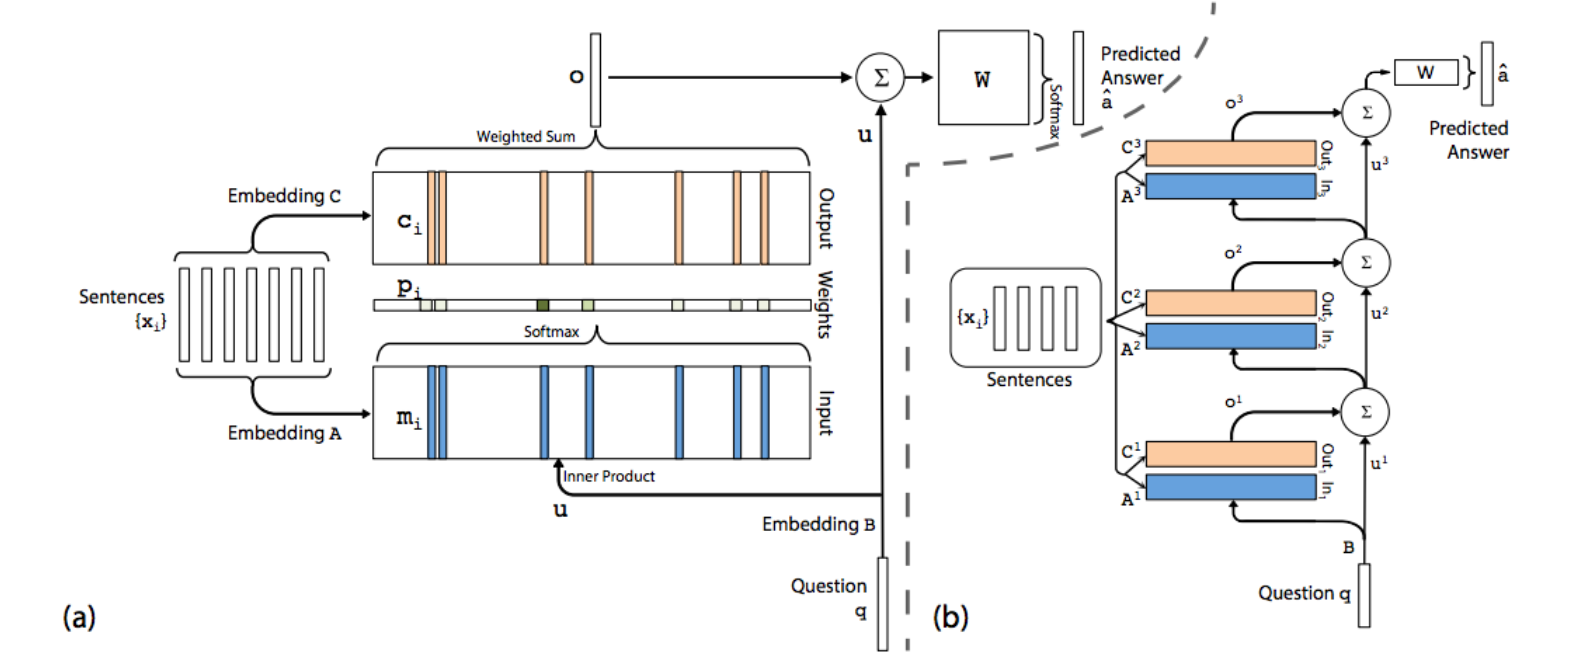
\includegraphics[width=0.8\linewidth]{model}
\end{figure}
\end{frame}

%------------------------------------------------

\begin{frame}
\frametitle{End-To-End Memory Networks Sukhbaatar et al 2015}
\begin{block}{Input Memory Representation}
\begin{gather*} 
	P(a|s,q) \\
	sl = max(story length) ; ql = max(query length); \\
	v = vocab size; D = Embedding dimension \\
	m[sl,D] = Embeddings[x(sl),A(v,D)]\\ 
	u[ql,D] = Embeddings[q(ql),B(v,D)]\\ 
	p[sl,ql] = Softmax(u * m)
\end{gather*}
\end{block}
\end{frame}

%------------------------------------------------

\begin{frame}
\frametitle{End-To-End Memory Networks Sukhbaatar et al 2015}
\begin{block}{Output Memory Representation}
\begin{gather*}
	c[sl,ql] = Embeddings[x(sl),C(v,ql)]\\
	o[sl,ql] = p * c \\
\end{gather*}
\end{block}

\begin{block}{Generate Answers}
\begin{gather*}
	a = Softmax(RNN([o,u]))
\end{gather*}
\end{block}

\begin{block}{Parameters to learn}
\begin{gather*}
	A,B,C,H
\end{gather*}
\end{block}

\end{frame}

\begin{frame}
\frametitle{Notes}
\begin{itemize}
\item Not able to train beyond 10K samples. Exhausts memory. 90M params to learn.
\item Pruning the story by finding similarities between question and story line pairs and pick top k. 
\item To compute similarity between two sentence, I found something called word mover's distance. Its basically a word embedding distance measure between distribution of words between sentence pairs. - "From Word Embeddings To Document Distances" by Kusner et al 2015
\item I have 15-20 percent validation accuracy in my runs, but Paper reports 80 percent for some categories. 
\item TODO: Parameter tunings, as much error analysis as possible.
\end{itemize}
\end{frame}

%------------------------------------------------

\begin{frame}
\frametitle{References}
\begin{itemize}
\item "End-To-End Memory Networks" by Sukhbaatar et al 2015
\item "From Word Embeddings To Document Distances" by Kusner et al 2015 
\item "WIKI READING : A Novel Large-scale Language Understanding Task over Wikipedia" by Hewlett et al 2016
\end{itemize}
\end{frame}
\end{document} 
